% subseccion 4.2
\subsection{Etapa 2: Búsqueda de Estudios}
Esta etapa presenta la estrategia de búsqueda usada en la revisión sistemática de la literatura. Esta estrategia se describe en detalle en las subsecciones~\ref{subsubsec:Definiendo la Estrategia de Busqueda} -- \ref{subsubsec:resultados-busqueda}. Ver figura~\ref{fig:etapa2}.

\begin{figure*}[tbp]
    \centering
    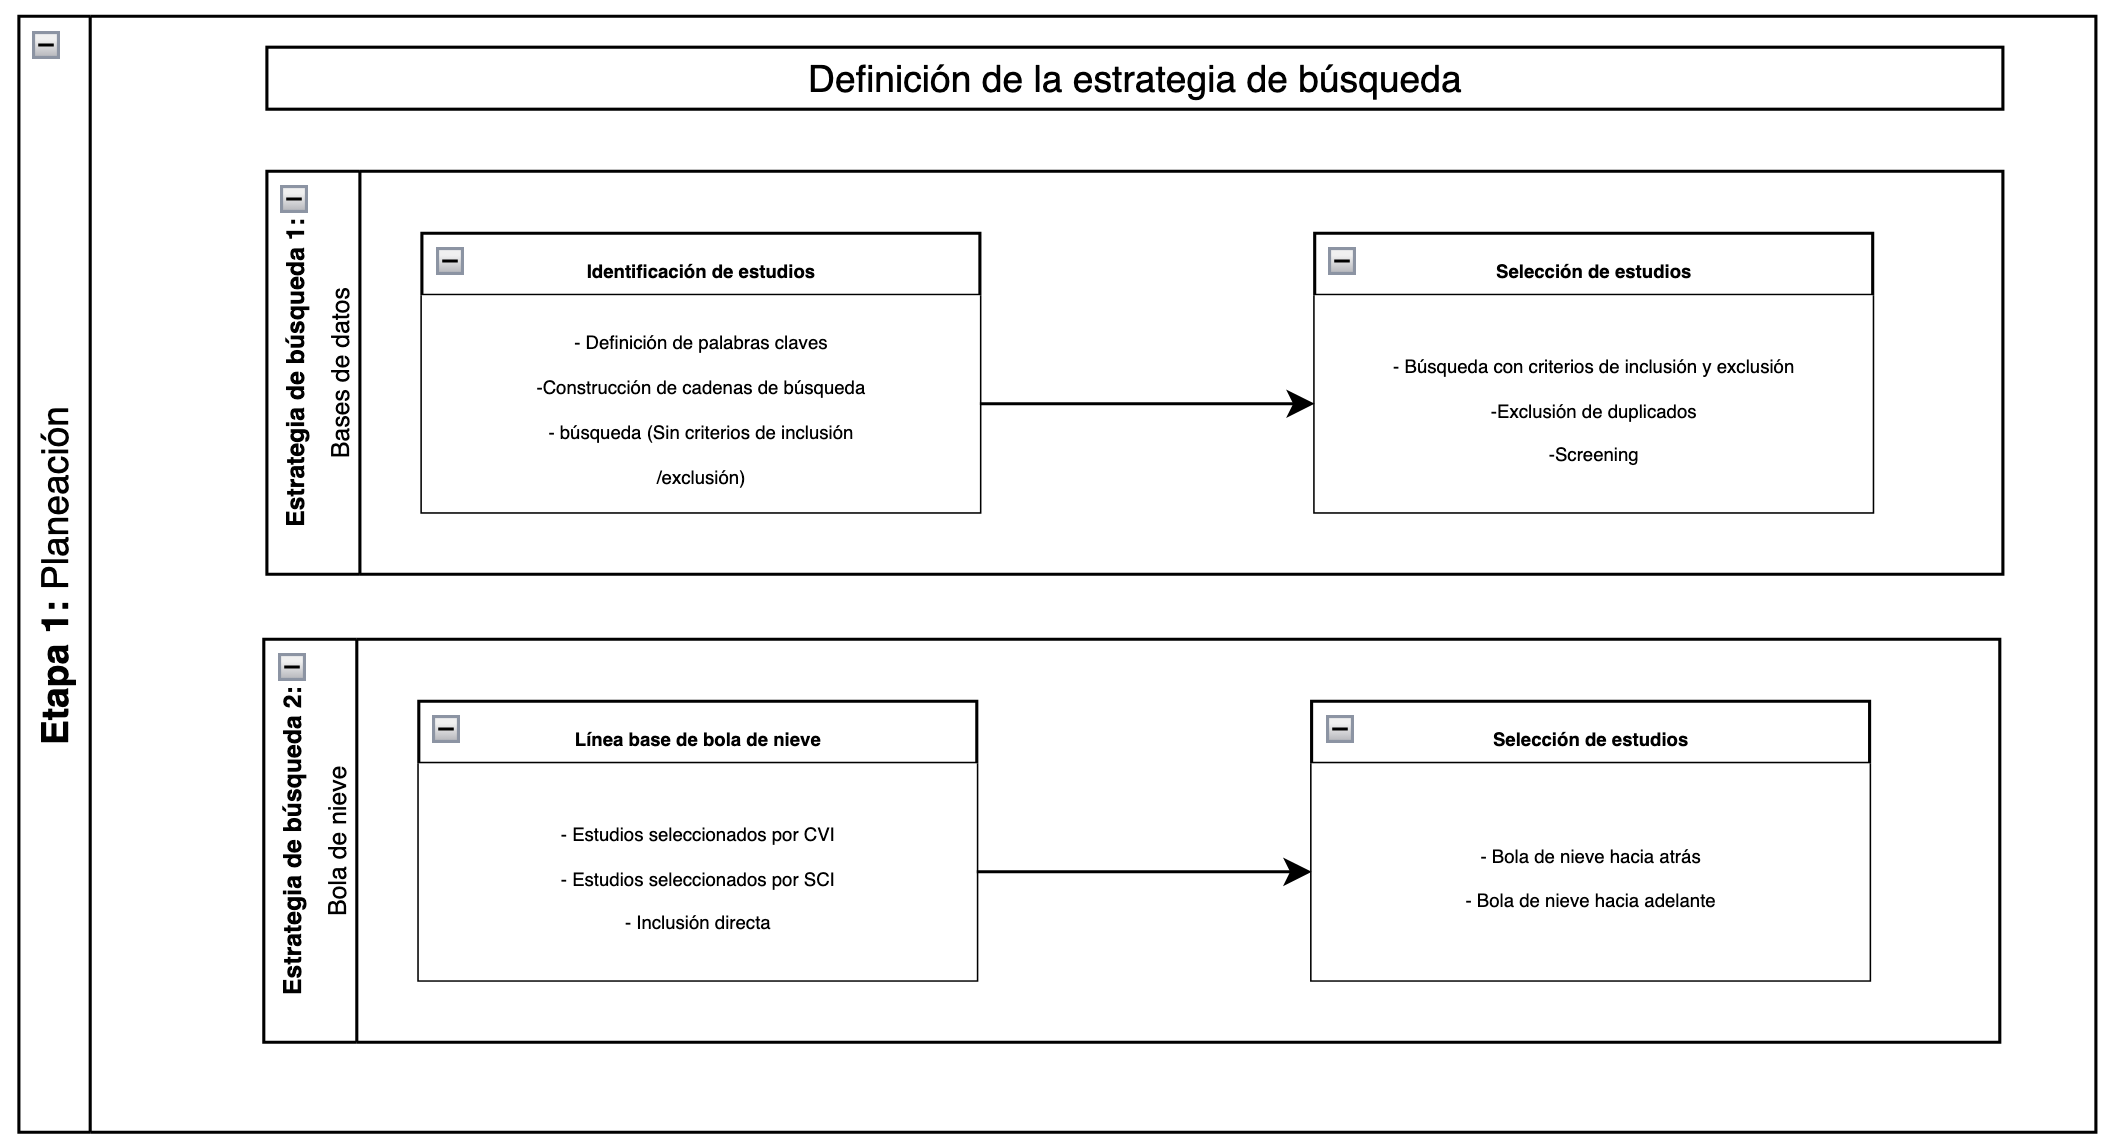
\includegraphics[width=0.8\textwidth]{resources/images/planeacion/estrategias-busqueda.png}
    \caption{Composición de la etapa de búsqueda de estudios}\label{fig:etapa2}
\end{figure*}
\mbox{}\\

%sub-subseccion 4.2.1 
\subsubsection{Definiendo la Estrategia de Búsqueda}\label{subsubsec:Definiendo la Estrategia de Busqueda}
\mbox{}\\
% Content for 4.2.1
Para la construcción de esta revisión de la literatura, se usó un enfoque híbrido. Con este enfoque se busca obtener mayor volumen de artículos indexados y con diferentes origenes. más allá de los proporcionados por las bases de datos.
En este sentido, se combinaron dos estrategias de búsqueda. La primer estrategia es la búsqueda en bases de datos y consiste en realizar una cadena de búsqueda automatizada en bases de datos académicas.~\cite{jalali2012systematic}.
La segunda estrategia es la denominada ``Bola de Nieve'' (Snowballing) y consiste en la búsqueda manual de artículos a partir de un conjunto base de artículos usando las referencias y las citas de los mismos. Esta estrategia se basa en la premisa de que los artículos relevantes citan otros artículos relevantes y, por lo tanto, permite encontrar artículos que no están indexados en las bases de datos académicas.~\cite{jalali2012systematic} y \cite{goodman1961snowball}.
\mbox{}\\
%sub-subseccion 4.2.2

\subsubsection{Estrategia de Búsqueda 1: Bases de Datos}
\mbox{}\\
Esta estrategia consta de 2 componentes. El primer componente es denominado ``Identificación de estudios''. Esto se enfoca en definir las palabras clave para construir las cadenas de búsqueda que conducen a completar las búsquedas en las bases de datos académicas.
El segundo componente es llamado ``Selección de estudios''. Se enfoca en aplicar varios criterios para refinar la búsqueda de resultados de estudios y así obtener el mayor valor del proceso de búsqueda. \\ \\

\begin{itemize}
    \item \textbf{Identificación de estudios: } En búsqueda de la viabilidad del estudio y por acuerdo de los autores, se limitó la búsqueda a cinco bases de datos académicas: \textit{ACM}, \textit{IEEE Xplore}, \textit{Springer}, \textit{Science Direct} y \textit{Taylor and Francis}. En esta parte del proceso es necesario establecer las palabras claves definidas antes y construir las cadenas de búsqueda específica para cada base de datos. Nuevamente se usó el modelo PICOC como guía metodológica para identificar términos claves o frases completas que se relacionan con las tecnologías de virtualización basadas en contenedores. En la construcción de estas cadenas de búsqueda se usaron sinónimos para ampliar el espectro de resultados. (Ver cuadro~\ref{tab:palabras-clave}).\\ 
    Las principales palabras clave identificadas fueron: \textit{Container-based virtualization}, \textit{Education}, \textit{Research}, \textit{Industry}. Para ampliar y refinar los resultados se usaron operadores booleanos como \textit{AND} y \textit{OR}. Además, se usaron comillas para buscar frases completas y paréntesis para agrupar términos relacionados. Finalmente, el conjunto de palabras clave seleccionadas para construir las cadenas de búsqueda se presenta en el cuadro~\ref{tab:keywords}.\\
    Para dirigir la búsqueda hacia la intercepción de los dominios de TI y la VBC se usó el operador booleano \textit{AND}. Una vez identificadas las palabras clave, se procedió con la construcción de las cadenas de búsqueda para cada base de datos, usando un proceso iterativo. El proceso de construcción de las cadenas de búsqueda consitió en realizar un proceso heúristico con las palabras clave, sinónimos y conceptos relacionados, haciendo uso de conjunciones y disyunciones conforme a las reglas de cada base de datos. Así, estas cadenas de búsqueda varían de acuerdo con las reglas de cada base de datos. Ver cuadro~\ref{tab:cadenas-busqueda}.\\

    Luego de la construcción de las cadenas de búsqueda, se procedió a ejecutarlas en cada base de datos. El cuadro~\ref{tab:resultados-busqueda-sin-criterio} muestra el conjunto de resultados obtenidos. Se identificó un total de 6530 preliminares, destacando que la base de datos \textit{Springer} es la que más resultados aportó, con un total de 4562 artículos, equivalente al 69.8\% del total.\\

    \item \textbf{Selección de estudios: } Para refinar los resutados obtenidos en este proceso, se aplicaron los criterios de inclusión y exclusión definidos en la etapa de planeación. La tabla~\ref{tab:resultados-busqueda-criterios} muestra el resultado de este paso. Se redujo el total de artículos a 976. Springer se mantuvo como la base de datos con mayor número de artículos, con un total de 592, equivalente al 60.65\% del total. De los 976 artículos seleccionados se eliminaron 274 artículos duplicados, dejando un total de 771 artículos únicos. De este nuevo conjunto de datos, se realizó una revisión llamada \textit{Screening}. Este proceso consistió en revisar el título, resumen y las palabras clave de cada artículo para determinar si están en el contexto de la investigación, esto significa que están alineado con las metas del estudio. 
    El proceso de \textit{Screening} permitió descartar 593 artículos debido a que se relacionaban con diferentes temas u otros enfoques que no aportaban valor a la investigación. Este proceso concluyó con un total de 110 estudios.
    De esta manera finaliza la estrategia de búsqueda en bases de datos, la figura \ref{fig:resumen-busqueda-bds} muestra un resumen de la metodología seguida en esta estrategia de búsqueda.\\
\end{itemize}

\begin{table}[tbp]
    \scriptsize % reduce tamaño del texto
    \centering
    \renewcommand{\arraystretch}{1.3}
    \begin{tabularx}{\columnwidth}{>{\centering\arraybackslash}m{0.18\columnwidth} >{\RaggedRight\arraybackslash}X}
        \hline
        \textbf{Aspecto} & \textbf{Descripción} \\
        \hline
        Población & VBC, Dominios de TI, Educación, Investigación, Extensión \\
        Intervención & Identificación, Clasificación \\
        Comparación & Tasa de éxito, Evidencia de uso \\
        Salida & Clasificación de trabajos relacionados con VBC en cada dominio de TI \\
        Contexto & Docencia, Investigación, Extensión \\
        \hline
    \end{tabularx}
    \caption{Palabras clave identificadas usando el modelo PICOC}\label{tab:palabras-clave}
\end{table}

\begin{table}[tbp]
    \scriptsize % reduce tamaño del texto
    \centering
    \renewcommand{\arraystretch}{1.3}
    \begin{tabularx}{\columnwidth}{>{\centering\arraybackslash}m{0.18\columnwidth} >{\RaggedRight\arraybackslash}X}
        \hline
        \textbf{Palabras clave} & \textbf{Sinónimos} \\
        \hline
        Container-based virtualization & Application virtualization, Docker, Lightweight Virtualization \\
        Education & Education System, Education Development, Higher Education \\
        Research & Research Group, Research Proposal \\
        Industry & IT Services, Technology Infrastructure, Cloud Computing \\
        \hline
    \end{tabularx}
    \caption{Palabras clave para la búsqueda en base de datos}\label{tab:keywords}
\end{table}

\begin{table*}[tbp]
    \scriptsize % reduce tamaño del texto
    \centering
    \renewcommand{\arraystretch}{1.3}
    \begin{tabularx}{\textwidth}{>{\raggedright\arraybackslash}X 
                                 >{\centering\arraybackslash}X 
                                 >{\centering\arraybackslash}X 
                                 >{\centering\arraybackslash}X 
                                 >{\centering\arraybackslash}X 
                                 >{\centering\arraybackslash}X}
        \hline
        \textbf{Criterio} & \textbf{ACM} & \textbf{IEEE} & \textbf{Science Direct} & \textbf{Springer} & \textbf{Taylor and Francis} \\
        \hline
        Resultados de cadenas de búsqueda solo con palabras clave & 189 & 426 & 4562 & 353 & 1000 \\
        Porcentaje de contribución & 2.89\% & 6.52\% & 69.86\% & 5.4\% & 15.31\% \\
        \hline
    \end{tabularx}
    \caption{Resultados de búsqueda por base de datos usando palabras clave}\label{tab:resultados-busqueda-sin-criterio}
\end{table*}

\begin{table*}[tbp]
    \scriptsize % reduce tamaño del texto
    \centering
    \renewcommand{\arraystretch}{1.3}
    \begin{tabularx}{\textwidth}{>{\raggedright\arraybackslash}X 
                                 >{\centering\arraybackslash}X 
                                 >{\centering\arraybackslash}X 
                                 >{\centering\arraybackslash}X 
                                 >{\centering\arraybackslash}X 
                                 >{\centering\arraybackslash}X}
        \hline
        \textbf{Criterio} & \textbf{ACM} & \textbf{IEEE} & \textbf{Science Direct} & \textbf{Springer} & \textbf{Taylor and Francis} \\
        \hline
        Resultados de cadenas de búsqueda solo con palabras clave & 48 & 134 & 46 & 592 & 156\\
        Porcentaje de contribución & 4.91\% & 13.72\% & 4.71\% & 60.65\% & 15.98\%\\
        \hline
    \end{tabularx}
    \caption{Resultados de búsqueda por base de datos usando palabras clave}\label{tab:resultados-busqueda-criterios}
\end{table*}

\newcolumntype{P}[1]{>{\raggedright\arraybackslash}p{#1}}

\begin{sidewaystable*}[htbp]
\centering
\scriptsize
\renewcommand{\arraystretch}{1.5}
\begin{adjustbox}{max width=\textwidth}
\begin{tabular}{|P{0.18\linewidth}|P{0.20\linewidth}|P{0.20\linewidth}|P{0.20\linewidth}|P{0.20\linewidth}|P{0.20\linewidth}|}
\hline
\textbf{Dominio / Base de Datos} & \textbf{ACM Digital Library} & \textbf{IEEE Xplore} & \textbf{ScienceDirect} & \textbf{SpringerLink}  & \textbf{Taylor \& Francis} \\
\hline
\textbf{Educación AND VBC} 
& \tiny \texttt{(Title:(``Container-based virtualization'' OR ``Application virtualization'' OR ``Docker'' OR ``Lightweight Virtualization'') AND Title:(``Education'' OR ``Education System'' OR ``Education Development'' OR ``Higher Education'')) OR (Abstract:(``Container-based virtualization'' OR ``Application virtualization'' OR ``Docker'' OR ``Lightweight Virtualization'') AND Abstract:(``Education'' OR ``Education System'' OR ``Education Development'' OR ``Higher Education'')) OR (Keyword:(``Container-based virtualization'' OR ``Application virtualization'' OR ``Docker'' OR ``Lightweight Virtualization'') AND Keyword:(``Education'' OR ``Education System'' OR ``Education Development'' OR ``Higher Education''))} 
& \tiny \texttt{((``Abstract'': ``Container-based virtualization'' OR ``Abstract'': ``Application virtualization'' OR ``Abstract'': ``Docker'' OR ``Abstract'': ``Lightweight Virtualization'') AND (``Abstract'': ``Education'' OR ``Abstract'': ``Education System'' OR ``Abstract'': ``Education Development''  OR ``Abstract'': ``Higher Education'')) OR ((``Publication Title'': ``Container-based virtualization'' OR ``Publication Title'': ``Application virtualization'' OR ``Publication Title'': ``Docker'' OR ``Publication Title'': ``Lightweight Virtualization'') AND (``Publication Title'': ``Education'' OR ``Publication Title'': ``Education System'' OR ``Publication Title'': ``Education Development''  OR ``Publication Title'': ``Higher Education'')) OR ((``Author Keywords'': ``Container-based virtualization'' OR ``Author Keywords'': ``Application virtualization'' OR ``Author Keywords'': ``Docker'' OR ``Author Keywords'': ``Lightweight Virtualization'') AND (``Author Keywords'': ``Education'' OR ``Author Keywords'': ``Education System'' OR ``Author Keywords'': ``Education Development''  OR ``Author Keywords'': ``Higher Education''))} 
& \tiny \texttt{(``Container-based virtualization'' OR ``Application virtualization'' OR ``Docker'' OR ``Lightweight Virtualization'') AND (``Education'' OR ``Education System'' OR ``Education Development'' OR ``Higher Education'')} 
& \tiny \texttt{(title:(``Container-based virtualization'' OR ``Application virtualization'' OR ``Docker'' OR ``Lightweight Virtualization'') AND title:(``Education'' OR ``Education System'' OR ``Education Development'' OR ``Higher Education'')) OR (abstract:(``Container-based virtualization'' OR ``Application virtualization'' OR ``Docker'' OR ``Lightweight Virtualization'') AND abstract:(``Education'' OR ``Education System'' OR ``Education Development'' OR ``Higher Education'')) OR (keyword:(``Container-based virtualization'' OR ``Application virtualization'' OR ``Docker'' OR ``Lightweight Virtualization'') AND keyword:(``Education'' OR ``Education System'' OR ``Education Development'' OR ``Higher Education''))} 
& \tiny \texttt{(``Application virtualization'' OR ``Docker'' OR ``Lightweight Virtualization'' OR ``Docker Container'') AND (``Education System'' OR ``Education Sector'' OR ``Education Development'' OR ``Higher Education'')} \\
\hline

\hline
\textbf{Investigación AND VBC}
& \tiny \texttt{(Title:(``Container-based virtualization'' OR ``Application virtualization'' OR ``Docker'' OR ``Lightweight Virtualization'') AND Title:(``Research'' OR ``Research Group'' OR ``Research Proposal'')) OR (Abstract:(``Container-based virtualization'' OR ``Application virtualization'' OR ``Docker'' OR ``Lightweight Virtualization'') AND Abstract:(``Research'' OR ``Research Group'' OR ``Research Proposal'')) OR (Keyword:(``Container-based virtualization'' OR ``Application virtualization'' OR ``Docker'' OR ``Lightweight Virtualization'') AND Keyword:(``Research'' OR ``Research Group'' OR ``Research Proposal''))} 
& \tiny \texttt{((``Abstract'': ``Container-based virtualization'' OR ``Abstract'': ``Application virtualization'' OR ``Abstract'': ``Docker'' OR ``Abstract'': ``Lightweight Virtualization'') AND (``Abstract'': ``Research Group'' OR ``Abstract'': ``Research Proposal'')) OR ((``Publication Title'': ``Container-based virtualization'' OR ``Publication Title'': ``Application virtualization'' OR ``Publication Title'': ``Docker'' OR ``Publication Title'': ``Lightweight Virtualization'') AND (``Publication Title'': ``Research Group'' OR ``Publication Title'': ``Research Proposal'')) OR ((``Author Keywords'': ``Container-based virtualization'' OR ``Author Keywords'': ``Application virtualization'' OR ``Author Keywords'': ``Docker'' OR ``Author Keywords'': ``Lightweight Virtualization'') AND (``Author Keywords'': ``Research Group'' OR ``Author Keywords'': ``Research Proposal''))} 
& \tiny \texttt{(``Container-based virtualization'' OR ``Application virtualization'' OR ``Docker'' OR ``Lightweight Virtualization'') AND (``Research'' OR ``Research Group'' OR ``Research Proposal'')} 
& \tiny \texttt{(title:(``Container-based virtualization'' OR ``Application virtualization'' OR ``Docker'' OR ``Lightweight Virtualization'') AND title:(``Research'' OR ``Research Group'' OR ``Research Proposal'')) OR (abstract:(``Container-based virtualization'' OR ``Application virtualization'' OR ``Docker'' OR ``Lightweight Virtualization'') AND abstract:(``Research'' OR ``Research Group'' OR ``Research Proposal'')) OR (keyword:(``Container-based virtualization'' OR ``Application virtualization'' OR ``Docker'' OR ``Lightweight Virtualization'') AND keyword:(``Research'' OR ``Research Group'' OR ``Research Proposal''))} 
& \tiny \texttt{(``Application virtualization'' OR ``Docker'' OR ``Lightweight Virtualization'' OR ``Docker Container'') AND (``Specific Research Areas'' OR ``Research Group'' OR ``Research Proposal'' OR ``Research and Development'')} \\
\hline

\hline
\textbf{Industria AND VBC}
& \tiny \texttt{(Title:(``Container-based virtualization'' OR ``Application virtualization'' OR ``Docker'' OR ``Lightweight Virtualization'') AND Title:(``Industry'' OR ``IT Services'' OR ``Technology Infrastructure'' OR ``Cloud Computing'')) OR (Abstract:(``Container-based virtualization'' OR ``Application virtualization'' OR ``Docker'' OR ``Lightweight Virtualization'') AND Abstract:(``Industry'' OR ``IT Services'' OR ``Technology Infrastructure'' OR ``Cloud Computing'')) OR (Keyword:(``Container-based virtualization'' OR ``Application virtualization'' OR ``Docker'' OR ``Lightweight Virtualization'') AND Keyword:(``Industry'' OR ``IT Services'' OR ``Technology Infrastructure'' OR ``Cloud Computing''))} 
& \tiny \texttt{((``Abstract'': ``Container-based virtualization'' OR ``Abstract'': ``Application virtualization'' OR ``Abstract'': ``Docker'' OR ``Abstract'': ``Lightweight Virtualization'') AND (``Abstract'': ``Industry'' OR ``Abstract'': ``IT Services'' OR ``Abstract'': ``Technology Infrastructure'' OR ``Abstract'': ``Cloud Computing'')) OR ((``Publication Title'': ``Container-based virtualization'' OR ``Publication Title'': ``Application virtualization'' OR ``Publication Title'': ``Docker'' OR ``Publication Title'': ``Lightweight Virtualization'') AND (``Publication Title'': ``Industry'' OR ``Publication Title'': ``IT Services'' OR ``Publication Title'': ``Technology Infrastructure'' OR ``Publication Title'': ``Cloud Computing'')) OR ((``Author Keywords'': ``Container-based virtualization'' OR ``Author Keywords'': ``Application virtualization'' OR ``Author Keywords'': ``Docker'' OR ``Author Keywords'': ``Lightweight Virtualization'') AND (``Author Keywords'': ``Industry'' OR ``Author Keywords'': ``IT Services'' OR ``Author Keywords'': ``Technology Infrastructure'' OR ``Author Keywords'': ``Cloud Computing''))} 
& \tiny \texttt{(``Container-based virtualization'' OR ``Application virtualization'' OR ``Docker'' OR ``Lightweight Virtualization'') AND (``Industry'' OR ``IT Services'' OR ``Technology Infrastructure'' OR ``Cloud Computing'')} 
& \tiny \texttt{(title:(``Container-based virtualization'' OR ``Application virtualization'' OR ``Docker'' OR ``Lightweight Virtualization'') AND title:(``Industry'' OR ``IT Services'' OR ``Technology Infrastructure'' OR ``Cloud Computing'')) OR (abstract:(``Container-based virtualization'' OR ``Application virtualization'' OR ``Docker'' OR ``Lightweight Virtualization'') AND abstract:(``Industry'' OR ``IT Services'' OR ``Technology Infrastructure'' OR ``Cloud Computing'')) OR (keyword:(``Container-based virtualization'' OR ``Application virtualization'' OR ``Docker'' OR ``Lightweight Virtualization'') AND keyword:(``Industry'' OR ``IT Services'' OR ``Technology Infrastructure'' OR ``Cloud Computing''))} 
& \tiny \texttt{(``Application virtualization'' OR ``Docker'' OR ``Lightweight Virtualization'' OR ``Docker Container'') AND (``Industry'' OR ``IT Services'' OR ``Technology Infrastructure'' OR ``Cloud Computing'')} \\
\hline
\end{tabular}
\end{adjustbox}
\caption{Cadenas de búsqueda por dominio y base de datos}\label{tab:cadenas-busqueda}
\end{sidewaystable*}


\begin{figure*}[tbp]
    \centering
    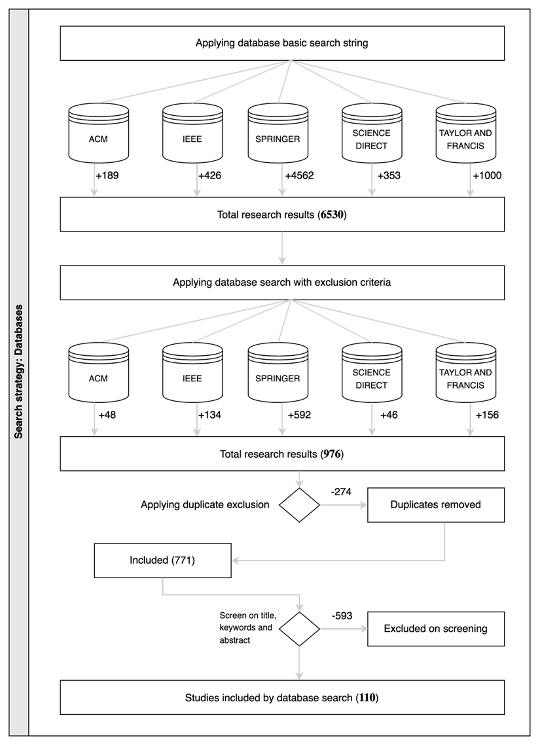
\includegraphics[width=0.8\textwidth]{resources/images/busqueda-estudios/busqueda-bd.png}
    \caption{Resumen de las actividades y resultados obtenidos en la estrategia de búsqueda en base de datos}\label{fig:resumen-busqueda-bds}
\end{figure*}

% sub-subsetion for 4.2.3
\subsubsection{Estrategia de Búsqueda 2: Bola de Nieve (Snowballing)}
La estrategia de búsqueda de bola de nieve inicia con la identificación del conjunto base de artículos. Este conjunto base se usó en la revisión y selección de artículos relevantes. La identificación consistió en revisar las referencias de cada artículo para identificar nuevos artículos (Bola de nieve hacia atrás). Similarmente, se revisaron los artículos que citan los artículos base (Bola de nieve hacia adelante) lo que requirió usar una base de datos que indique esta información. En ambos casos, se aplicaron los criterios de inclusión y exclusión definidos en la etapa de planeación \cite{10.1145/2601248.2601268}. \\ \\
Esta estrategia se realizó en dos pasos. El primer paso es llamado \textit{Construcción de la línea base} y tiene como objetivo establecer los artículos sobre los cuales se realizarán un análisis de citas y referencias. Para la construcción de este conjunto de estudios, se usó varios criterios basados en el CVI \textit{(Content Value Index)}, SCI \textit{(Study Citation Index)}, además de usar el criterio de inclusión directa. El segundo paso es llamado \textit{Selección de estudios} y se enfoca en el análisis de la referencias \textit{(Backward Snowballing)} y citas \textit{(Forward Snowballing)} de cada artículo. \\ \\
La construcción de la línea base inicia con los 110 artículos obtenidos en la estrategia de búsqueda en bases de datos. De estos, se seleccionaron 24 artículos aplicando el critero de calidad SCI. La elección de este criterio se justifica en el hecho de que este criterio no depende de la valoración de los autores, sino que se basa en la cantidad de citas que recibe un artículo siendo este un indicador no subjetivo. El resultado de este paso es un total de 24 artículos seleccionados para la línea base. Los 24 artículos seleccionados se obtuvieron de hacer una análisis de frecuencia en las citas y extraer el primer cuartil (Q1) de los artículos más citados.\\ \\
Como parte del proceso del SMS, es posible agregar estudios por inclusión directa. La inclusión directa aporta flexibilidad al proceso de búsqueda permitiendo añadir artículos que los autores consideran relevantes para el estudio. En este sentido, se agregaron 2 artículos por inclusión directa, lo que llevó a un total de 26 artículos en la línea base.\\ \\
Luego de la construcción de la línea base, se procedió con el análisis de las referencias, lo que aportó un total de 495 artículos nuevos. El proceso de búsqueda hacia adelante fue realizado haciendo uso de Google Scholar, quien proporciona información sobre las veces que que un artículo se ha citado y siguiendo las practicas de~\cite{8747000}. 
Con respecto a la búsqueda hacia atrás fue un total de 87 nuevos artículos.\\

Se procedió a eliminar 14 duplicados entre los resultados de las búsquedas hacia atrás y hacia adelante. Acto seguido, se realizó nuevamente el \textit{Screening}. Este proceso de \textit{Screening}, al igual que el anterior, revisó el título, resumen y palabras claves, permitiendo reducir a 116 los artículos seleccionados usando estrategia de búsqueda. Ver figura~\ref{fig:resumen-busqueda-snowballing} para un resumen de la estrategia de búsqueda bola de nieve.\\ \\
\mbox{}

\begin{figure*}[tbp]
    \centering
    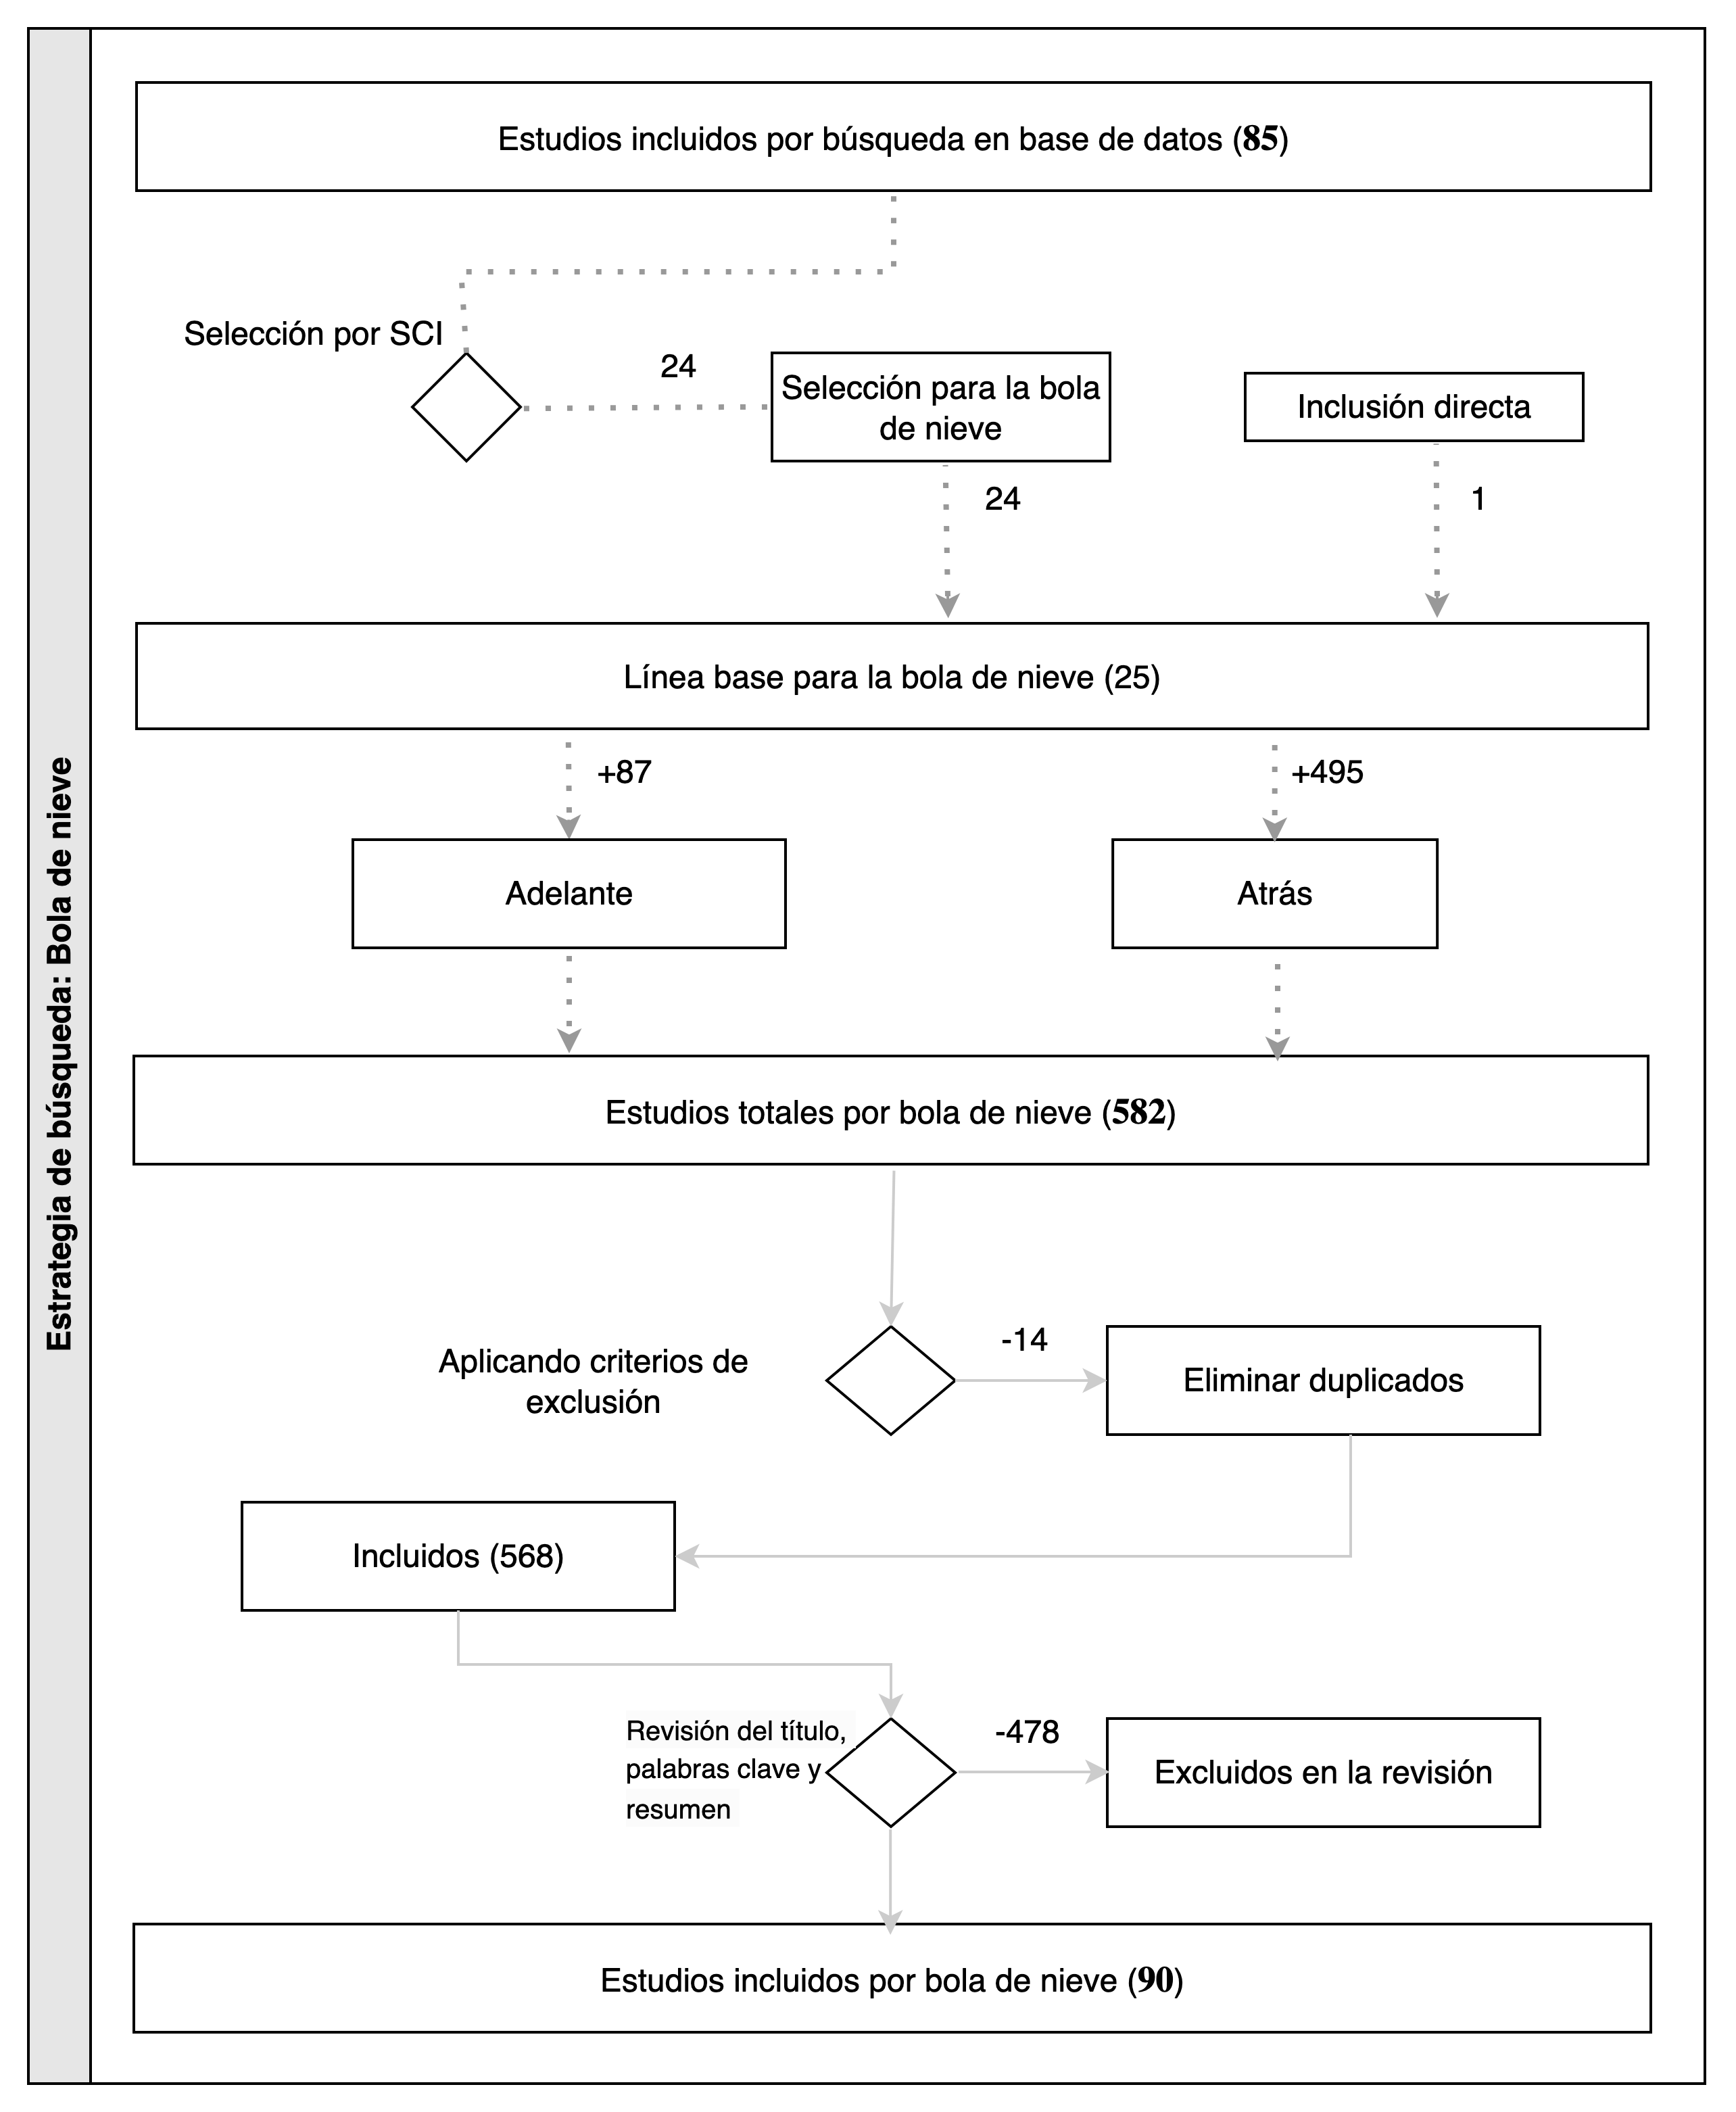
\includegraphics[width=0.8\textwidth]{resources/images/busqueda-estudios/busqueda-snowball.png}
    \caption{Resumen de la estrategia de búsqueda - Bola de nieve}\label{fig:resumen-busqueda-snowballing}
\end{figure*}

\begin{table}[htbp]
\renewcommand{\arraystretch}{1.3}
\begin{tabularx}{\columnwidth}{
    >{\centering\arraybackslash}m{0.3\textwidth}
    >{\centering\arraybackslash}X
    >{\centering\arraybackslash}m{0.15\textwidth}
}
\toprule
\textbf{Estrategia} & \textbf{Estudios} & \textbf{\%} \\
\midrule
Bases de Datos & 110 & 48.67\% \\
Bola de Nieve & 116 & 51.33\% \\
\textbf{Total} & \textbf{226} & \textbf{100\%} \\
\bottomrule
\end{tabularx}
\caption{Resultados de la búsqueda de estudios}\label{tab:resultados-busqueda}
\end{table}

% sub=-subsection 4.2.4
\subsubsection{Resultados de la Búsqueda de Estudios}\label{subsubsec:resultados-busqueda}
\mbox{}\\
Finalmente, se resumen la búsqueda de artículos en 110 estudios obtenidos a través de bases de datos académicas y 116 estudios identificados mediante bola de nieve, para un total de 226 estudios identificación. Ver cuadro~\ref{tab:resultados-busqueda}
\mbox{}\\